% ====================================================================
%+
% SECTION NAME:
%    lss.tex
%
% CHAPTER:
%    cosmology.tex
%
% ELEVATOR PITCH:
%    Large Scale Structure, Weak Lensing, and Clusters all require
%    survey uniformity in the static 10-year survey.  A key contributor
%    to this is the pattern of dithers adopted.
%
% AUTHORS:
%   Eric Gawiser (@egawiser)
%-
% ====================================================================
\newcommand{\sigmaOS}[0]{$\sigma_{\mathrm{C_{\ell, {OS}}}}$}
\newcommand{\CellOS}[0]{$C_{\ell, \rm{OS}}$}
\newcommand{\statFloor}[0]{$\Delta C_\ell$}
\newcommand{\delobs}[0]{\delta_{\mathrm{obs},i}}
\newcommand{\dellss}[0]{\delta_{\mathrm{LSS},i}}
\newcommand{\delos}[0]{\delta_{\mathrm{OS},i}}
\newcommand{\ev}[1]{\left < {#1} \right >}

\section{Large-Scale Structure: Testing Dither Patterns and Timescales to Improve Survey Uniformity}
\def\secname{lss}\label{sec:\secname}

\credit{HumnaAwan},
\credit{egawiser},
\credit{pkurczynski},
\credit{rhiannonlynne}

Three of the key cosmology probes available with LSST represent ``static science'', i.e., insensitive to time-domain concerns.  These are Weak Lensing, Large-Scale Structure, and Galaxy Clusters.  Nonetheless, due to the need to track and correct for the survey window function for these probes, cosmology with LSST will benefit from achieving survey depth as uniform as possible over the WFD area.  OpSim tiles the sky in hexagons inscribed within the nearly-circular LSST FOV. It has been shown in \citet{CarrollEtal2014} that the default LSST survey strategy implemented in OpSim leads to a strongly non-uniform honeycomb pattern due to overlapping regions on the edges of the hexagons receiving nearly double the observing time.  A pattern of large dithers, i.e. telescope-pointing offsets on the scale of the LSST FOV, greatly reduces these overlaps, leading to an increase in the median survey depth in each filter by 0.08 magnitudes.

In this section, we report the results from an investigation into different types of dithers, varying both in terms of the timescales on which dithers are implemented as well as the geometry of the dither positions. The results discussed largely follow the analysis in \citet{AwanEtal2016}, except that here we use the $i$-band-relative mock catalogs and magnitude cuts (as opposed to the $r$-band), and analyze the impacts of different observing strategies using the new baseline cadence \opsimdbref{db:baseCadence} and two other cadences. We also discuss the quantification of the effectiveness of a given observing strategy as a Figure of Merit.

% ====================================================================
% Subsection: Dither Patterns and Timescales
% ====================================================================
\subsection{Dither Patterns and Timescales}
\label{sec:\secname:strategies}
As in \citet{AwanEtal2016}, we consider three timescales to capture the range of time intervals on which dithers can be implemented: by visit, by night, and by season. Both visit and night timescales are well-defined in OpSim \citep[see]{IvezicEtal2008}. For the seasons, we use the \href{https://github.com/lsst/sims_maf/blob/master/python/lsst/sims/maf/stackers/generalStackers.py}{SeasonStacker}, which assigns a season to every observation by tracking when each field's RA is overhead in the middle of the day. The season assignment leads to 11 seasons, and for our purposes, we treat the 0th and 10th seasons the same by assigning them the same dither position.

Another variation in the implementation timescale is added by dithering each field independently as opposed to dithering all fields collectively. For instance, FieldPerNight timescale assigns a new dither position to a field when it is observed on a new night, while PerNight implementation assigns a new dither to all fields every night regardless of whether a particular field is observed or not.

In \citet{AwanEtal2016}, we study five different geometries for the dither positions, where one geometry is specifically for PerSeason assignment and the rest are implemented on three timescales, namely FieldPerVisit, FieldPerNight, and PerNight. Here, we focus only on three combinations of the different geometries and timescales as an illustration of the impacts of these combinations: RepulsiveRandomDitherFieldPerVisit, FermatSpiralDitherPerNight,  and PentagonDitherPerSeason. These geometries are shown in \autoref{fig: dithGeometries}, adapted from Figure 1 in \citet{AwanEtal2016}.

\begin{figure*}[!htb]
      \centering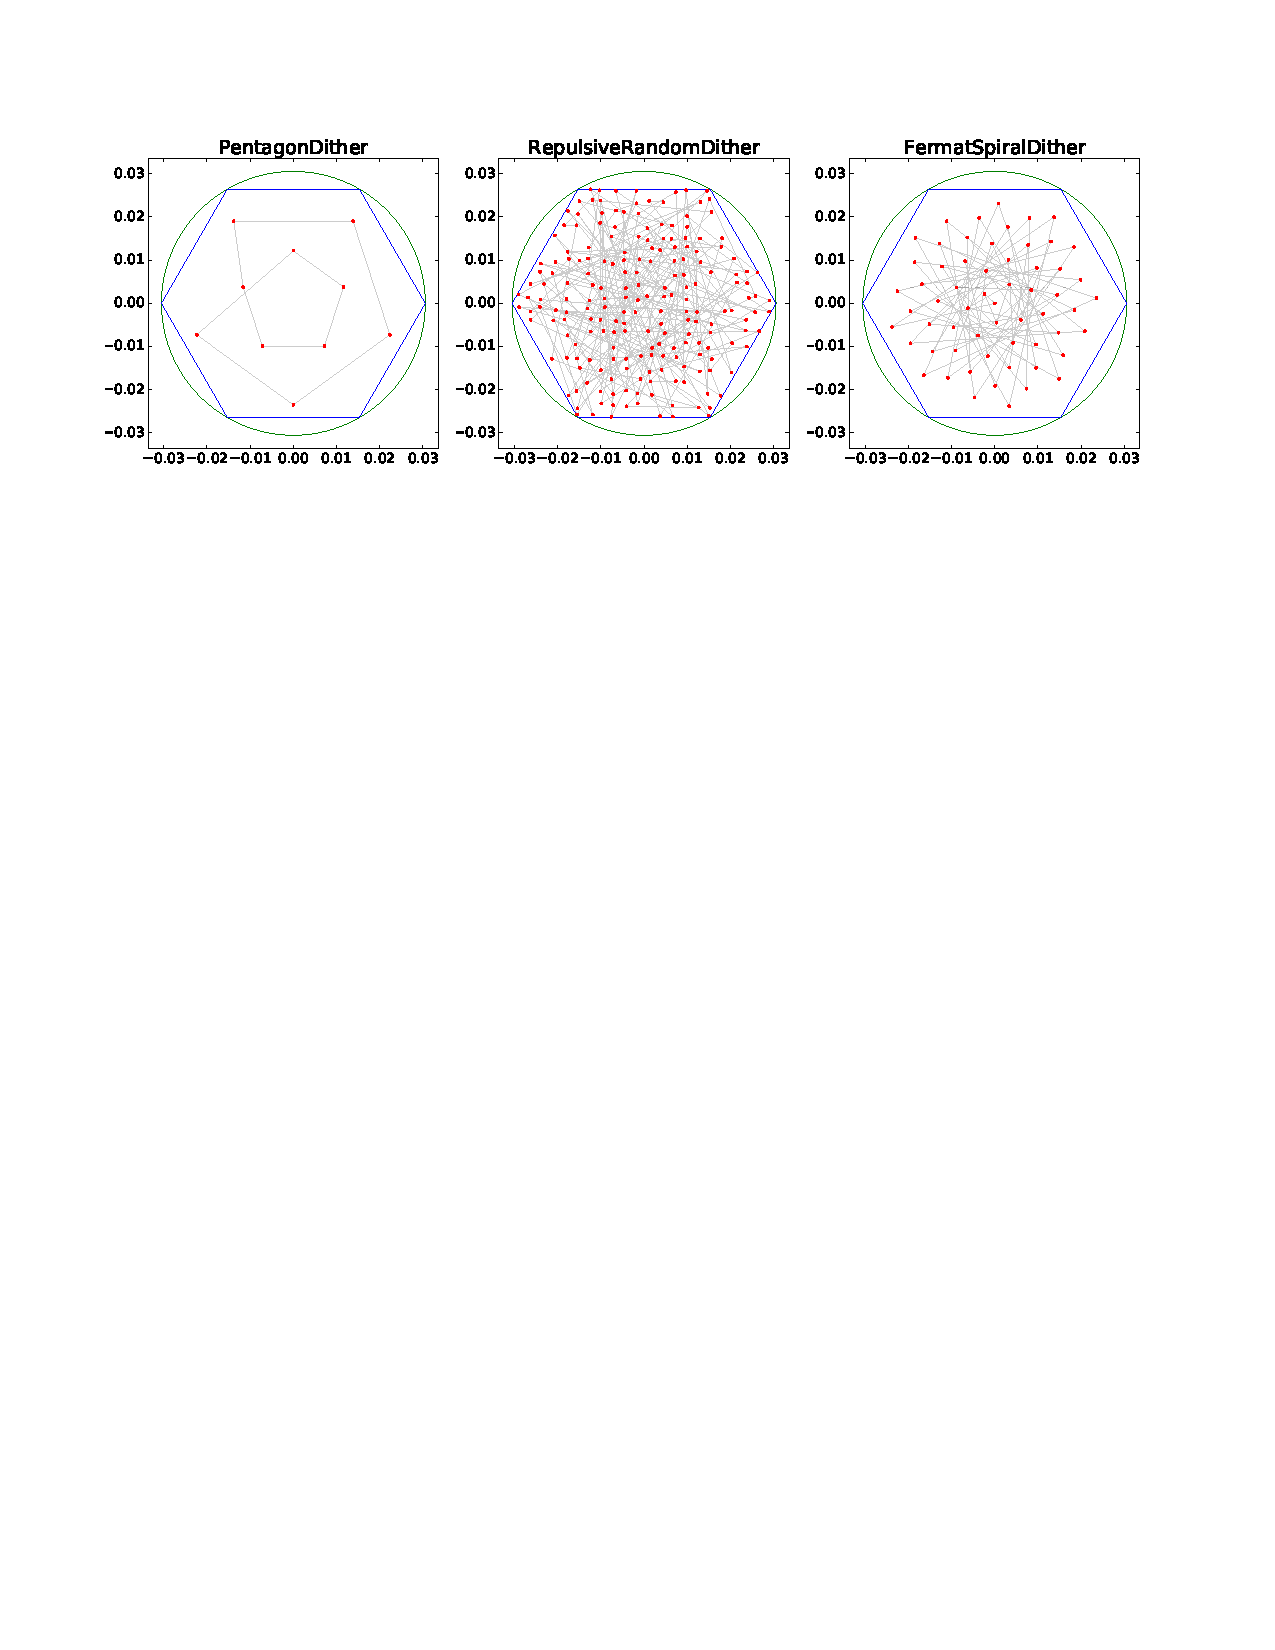
\includegraphics[width=\linewidth, trim={25 570 25 50},clip=true]{figs/awan_dithGeometries.pdf}
\caption{Dither geometries implemented for various timescales. PentagonDither is implemented only on PerSeason timescale, while the rest are implemented on FieldPerVisit, FieldPerNight, and PerNight timescales. Here the green curve is the LSST FOV of radius 0.305 radians; the blue hexagon represents the hexagonal tiling of the sky originally adopted for the undithered observations; and the red points are the dithers. The axes are in radians.}
\label{fig: dithGeometries}
\end{figure*}

Here we note that all the dithers are restricted to lie within the hexagons inscribed in the 3.5$^\circ$ LSST FOV, and that we continue with the naming scheme [Geometry]Dither[Field]Per[Timescale], where the absence of the tag `Field' implies that all fields are assigned the same dither.

% ====================================================================
% Subsection: Metrics
% ====================================================================
\subsection{Metrics}
\label{sec:\secname:metrics}
Our first metric is the \href{https://github.com/lsst/sims_maf/blob/master/python/lsst/sims/maf/metrics/simpleMetrics.py}{CoaddM5Metric}, which we use to calculate the coadded 5$\sigma$ depth resulting from various observing strategies. This allows us to compare the artifacts in the coadded depth induced by the observing strategy. Then we account for the dust extinction, using \href{https://github.com/lsst/sims_maf/blob/master/python/lsst/sims/maf/metrics/exgalM5.py}{ExGalM5Metric}, before estimating the number of galaxies in each pixel at a particular depth. For this purpose, we use a mock LSST catalog \citep{MunozEtal2015} to estimate the power law coefficients for each redshift bin, converting the depth into an estimated number of galaxies for each pixel \citep[Eq. 2]{AwanEtal2016}:
\begin{equation}
	N_{\mathrm{gal}}= 0.5\int_{-\infty}^{m_\mathrm{{max}}} {\mathrm{erfc}[a(m-5\sigma_{\mathrm{stack}})] 10^{c_1m + c_2}dm}
	\label{eq: Ngal}
\end{equation}

Here the \texttt{erfc} function accounts for incompleteness while the constants c$_1$ and c$_2$ are determined from the mock catalog. $m_{\mathrm{max}}$ specifies the magnitude cut, and we modify both $m_\mathrm{{max}}$ and c$_2$ to account for colors (assumed to be $u-g= g-r= r-i= 0.4$). This calculation is carried out using the \href{https://github.com/humnaawan/sims_maf_contrib/blob/master/mafContrib/galaxyCountsMetric_extended.py}{GalaxyCountMetric}.

We then account for the effects of photometric calibrations in our estimated number of galaxies. As discussed in \citet{AwanEtal2016}, we model the calibration uncertainties using a simple ansatz relating the systematic errors in each pixel to the seeing in that pixel (relative to the average seeing across the survey region; $\Delta s_{i}$)  and number of observations $N_{\mathrm{obs},i}$:
\begin{equation}
	\Delta_{i}= \frac{k \Delta s_{i}}{\sqrt{N_{\mathrm{obs}, i}}}
\end{equation}
where $k$ is a constant such that $\sigma_{\Delta_i}$ matches the LSST photometric calibration goal of 1$\%$  \citep{2009arXiv0912.0201L}. Since the calibration uncertainties are pixel-dependent, we use the \href{https://github.com/humnaawan/sims_maf_contrib/blob/master/mafContrib/galaxyCounts_withPixelCalibration.py}{pseudo-GalaxyCountsMetric}, which handles pixel-by-pixel calculation to modify the upper limit in the integral in \autoref{eq: Ngal} to be $m_{\mathrm{max}} + \Delta_{i}$, thereby accounting for the fluctuations in the galaxy counts due to the calibration errors. We then calculate the fluctuations in the galaxy counts in each pixel, $\delta_i= \Delta N_i/\overline{N}$.

% ====================================================================
% Subsection: Figure of Metric
% ====================================================================
\subsection{Figure of Merit}
\label{sec:\secname:FoM}
As derived and discussed in \citet{AwanEtal2016}, the spurious power from the artificial fluctuations in the galaxy counts induced by the observing strategy (OS) represents a bias in our measurement of the LSS. Hence, the uncertainty in this bias becomes the limiting factor in our ability to correct for the OS-induced structure. More quantitatively, for an optimized LSS study, the OS-induced uncertainties, \sigmaOS, must be subdominant to the statistical uncertainty \statFloor\ inherent to the measured power spectrum due to ``cosmic variance'' \citep{Dodelson}:
\begin{equation}
	\Delta C_\ell= C_{\ell,\mathrm{LSS}} \sqrt{\frac{2}{f_{\mathrm{sky}} (2\ell + 1)}}
	\label{eq: statFloor}
\end{equation}
where $f_{\rm{sky}}$ is the fraction of the sky observed, accounting for the reduction in the observed information due to incomplete sky coverage.

Since we do not include any input LSS in our pipeline, the power spectrum we measure for any given band is due to the OS-induced power, \CellOS, for that band. Modeling the overall OS-induced bias as an average across $ugri$ bands, we calculate the OS-induced uncertainties \sigmaOS\ as the standard deviation across \CellOS\ for $ugri$ bands to account for the effects of detecting the galaxy catalog through various bands. We then compare these uncertainties with the statistical floor for various redshift bins, where the statistical floor is based on the galaxy power spectra calculated using the code from \citet{Zhan2006}, which we pixelize to match the HEALPix resolution to account for the finite angular resolution of our simulations.

To quantify the effectiveness of each observing strategy in minimizing \sigmaOS, we construct a Figure of Merit (FoM) as the ratio of the ideal-case uncertainty in the measured power spectrum and the uncertainty where shot noise and OS-induced structure also play a role:
\begin{equation}
	\mathrm{FoM} = \sqrt{\frac{\sum\limits_\ell{\left({\sqrt{\frac{2}{f_{\mathrm{sky, max}} (2\ell + 1)}}C_{\ell, \mathrm{LSS}}} \right)}^2}{\sum\limits_\ell \left[{ \left( { \sqrt{\frac{2}{f_{\mathrm{sky}} (2\ell + 1)}}\left\{{C_{\ell, \mathrm{LSS}} + \frac{1}{\bar{\eta}}} \right\}  } \right ) ^2 + \sigma_{C_{\ell,\mathrm{OS}}}^2  }\right]}}
\label{eq: FoM}
\end{equation}
Here, $\bar{\eta}$ is the surface number density in steradians$^{-1}$, and the term containing it accounts for the contribution from the shot noise to the measured signal \citep{HutererEtal2001,Jing2005}. This FoM measures the percentage of ideal-case information that can be measured in the presence of systematics. We note that the shot noise is negligible even for the shallowest (10-year) surveys we consider.

We define the ideal-case as being based on the largest coverage of the sky with LSST, i.e., $f_{\rm{sky, max}}$ is the largest WFD coverage with the baseline cadence. For \opsimdbref{db:baseCadence}, the observing strategy with RepulsiveRandomDitherFieldPerVisit dithers leads to the largest $f_{\rm{sky}}$ ($\sim 39.5\%$). Note that this fraction is calculated after masking the shallow borders of the main survey; for details, see \citet{AwanEtal2016}. %Therefore, we fix the $f_{\rm{sky, best}}$ to be $39.5\%$ and compare the the different observing strategies and cadences relative to it. 

% ====================================================================
% Subsection: A Comment on Terminology
% ====================================================================
\subsection{A Comment on Terminology}
For clarity, we make a note on the terminology we have introduced. Strictly speaking, the bias caused by the observing strategy is a window function bias, as the survey window function ($W_i$) accounts for the effective survey geometry which scales the fluctuations in the galaxy counts in each pixel: $1+\delobs= W_i(1+\dellss)$. Comparing this with Equation 4 in \citet{AwanEtal2016}, $1+\delobs= (1+\delos)(1+\dellss)$, we see that the OS-induced bias is directly related to the window function: $1 + \delos= W_i$

Then, for the total power, we have
\begin{equation}
\ev{\delobs^2}=\ev{\dellss^2}\ev{(1 + \delos)^2}+ \ev{\delos^2}=\ev{\dellss^2}\ev{W_i^2}+ \ev{(W_i-1)^2}
\end{equation}
where the first equality is based on Equation 6 in \citet{AwanEtal2016} and the second one holds given the relation between $\delos$ and $W_i$. Since the OS-induced bias $\delos^2=  (W_i-1)^2$, the uncertainties in the OS-induced bias are the window function uncertainties.

Generally the window function is assumed to be known perfectly and its uncertainties are not explicitly identified as such. To avoid confusion and focus on the window function uncertainties arising from the observing strategy, we continue using the term OS-induced bias and its uncertainties in favor of window function and its uncertainties.

% ====================================================================
% Subsection: OpSim Analysis and Results
% ====================================================================
\subsection{OpSim Analysis and Results}
\label{sec:\secname: analysis}
For the purposes of our analysis, we use HEALPix resolution of $N_\mathrm{_{side}}= 256$, effectively tiling each $3.5^\circ$ FOV with about 190 HEALPix pixels. Using the metrics discussed in \autoref{sec:\secname:metrics}, we analyze \sigmaOS\ from various observing strategies. First we present the results for the baseline cadence, \opsimdbref{db:baseCadence}.

\begin{figure*}[!htb]
      \centering\hspace*{-3em}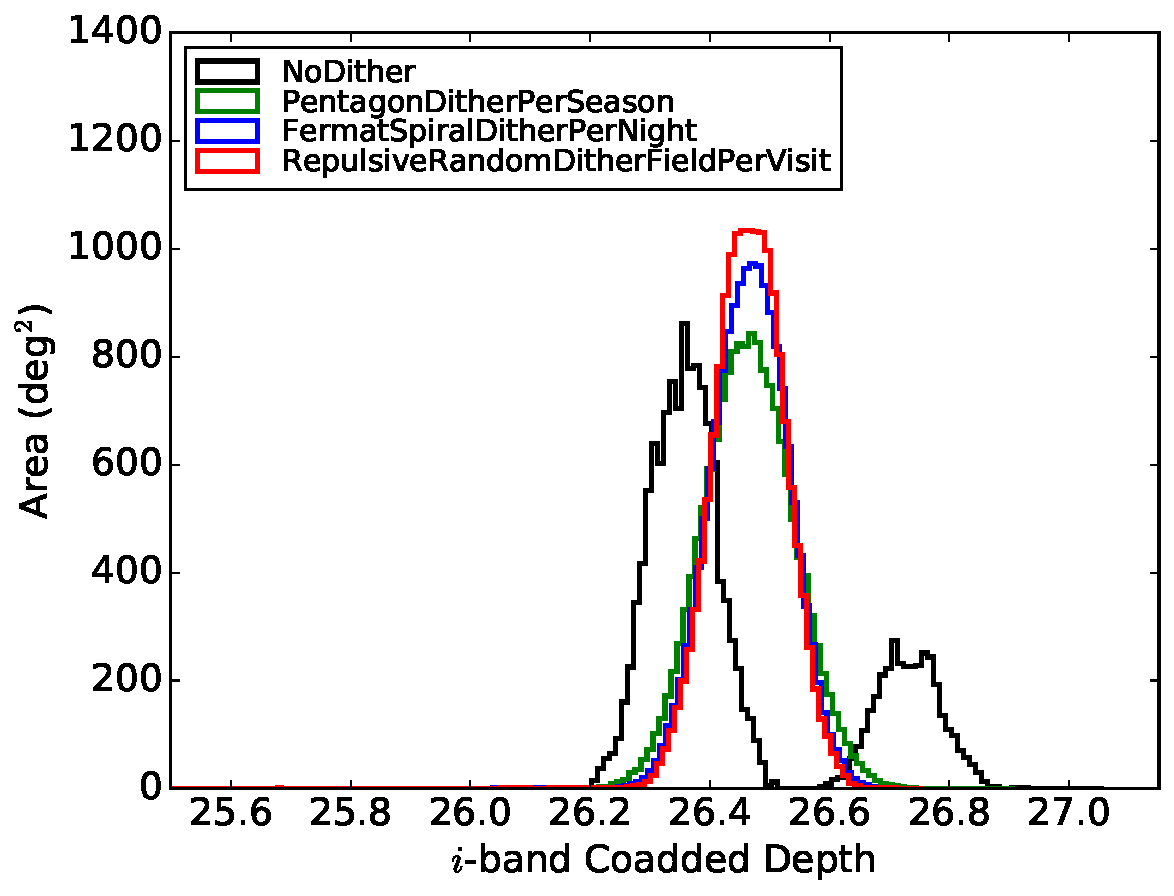
\includegraphics[width=0.6\linewidth]{figs/awan_coaddHistogram.pdf}
      \vspace*{-1em}
\caption{Histogram for the $i$-band coadded 5$\sigma$ depth after the full, 10-year survey.}
\label{fig: coaddHistogram}
\end{figure*}

\autoref{fig: coaddHistogram} shows the histogram for the $i$-band coadded 5$\sigma$ depth from \opsimdbref{db:baseCadence} for the four observing strategies. We observe a bimodal distribution for the undithered survey -- the deeper depth mode corresponds to the overlapping regions between the hexagons, while the rest of the survey contributes to the shallower mode. In contrast, all dithered surveys lead to unimodal distributions as the overlapping regions between the fields change frequently, leading to more uniformity. We also note that frequent dithering leads to deeper regions as we observe more peaked histograms for FieldPerVisit and PerNight strategies.

\autoref{fig: coaddSkymaps} shows the plots for the $i$-band coadded 5$\sigma$ depth for the observing strategies. As in \citet{AwanEtal2016}, we find that the undithered survey leads to a strong honeycomb pattern which is much weaker in all of the dithered surveys. We again observe that the dithered surveys are deeper than the undithered survey in terms of the median depth across the survey region.

\begin{figure*}[!htb]
      \centering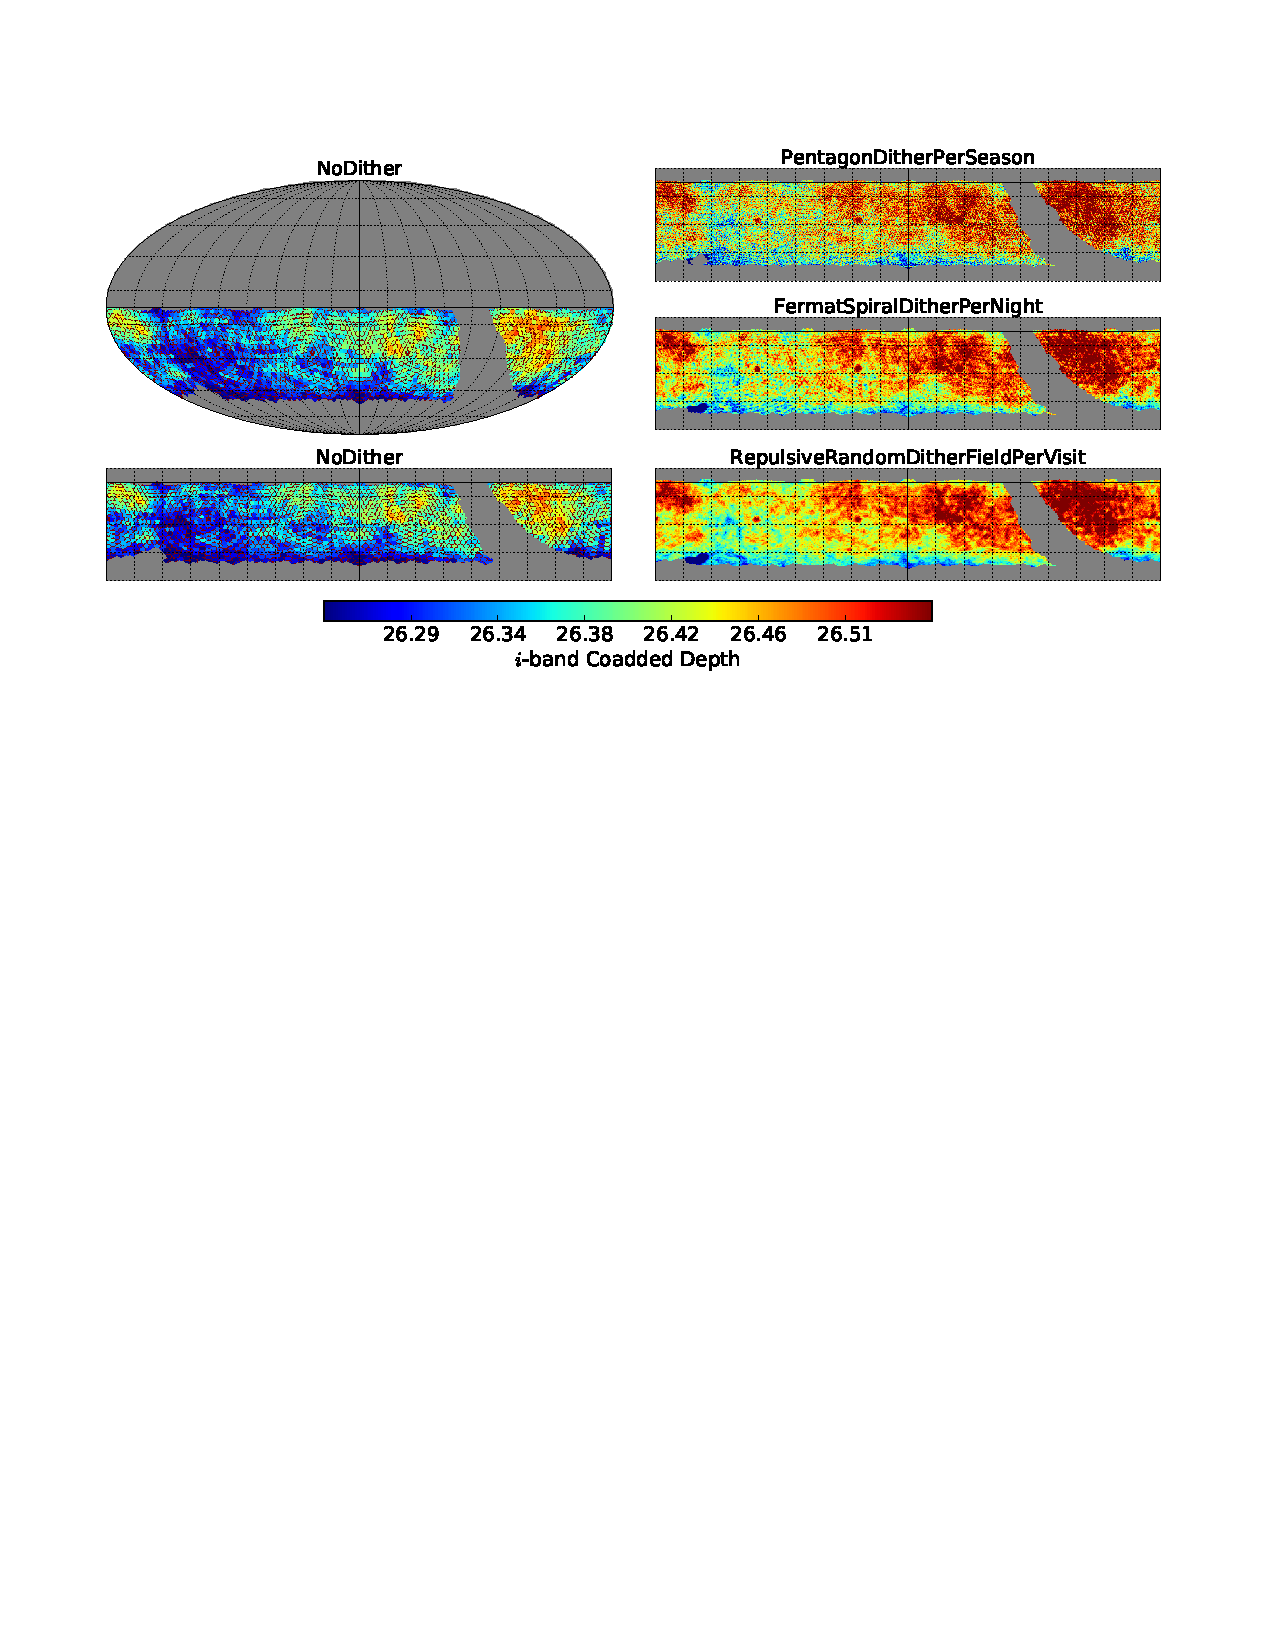
\includegraphics[width=\linewidth, trim={50 470 55 70},clip=true]{figs/awan_minion1016_coaddSkymaps.pdf}
\caption{Plots for the $i$-band coadded 5$\sigma$ depth based on \opsimdbref{db:baseCadence} for various observing strategies. The top left plot shows the Mollweide projection for NoDither while the bottom left shows the corresponding Cartesian projection, restricted to $180^\circ>$RA$>-180^\circ$ (left-right), $-70^\circ<$Dec$<10^\circ$ (bottom-top). Only the latter is shown for the rest of the strategies. }
\label{fig: coaddSkymaps}
\end{figure*}

In order to quantify the angular characteristics observed in the skymaps, we calculate the angular power spectra corresponding to the skymaps for the $i$-band coadded 5$\sigma$ depth. \autoref{fig: coaddPowerSpectrum} shows these spectra for the four observing strategies. We observe a sharp reduction in the artificial power in the dithered surveys when compared to the undithered one: the strong honeycomb pattern in the undithered survey leads to a large peak around $\ell\sim150$, while the peak is about 10 times weaker in the dithered surveys. We do, however, observe variations amongst the various dither strategies: while RepulsiveRandom dithers lead to small power for all timescales, PerSeason dithers lead to large power on larger angular scales, and both PerSeason and FermatSpiral lead to large power around $\ell\sim150$ (which still is $<10\times$ the corresponding peak from the undithered survey).

\begin{figure*}[!htb]
      \centering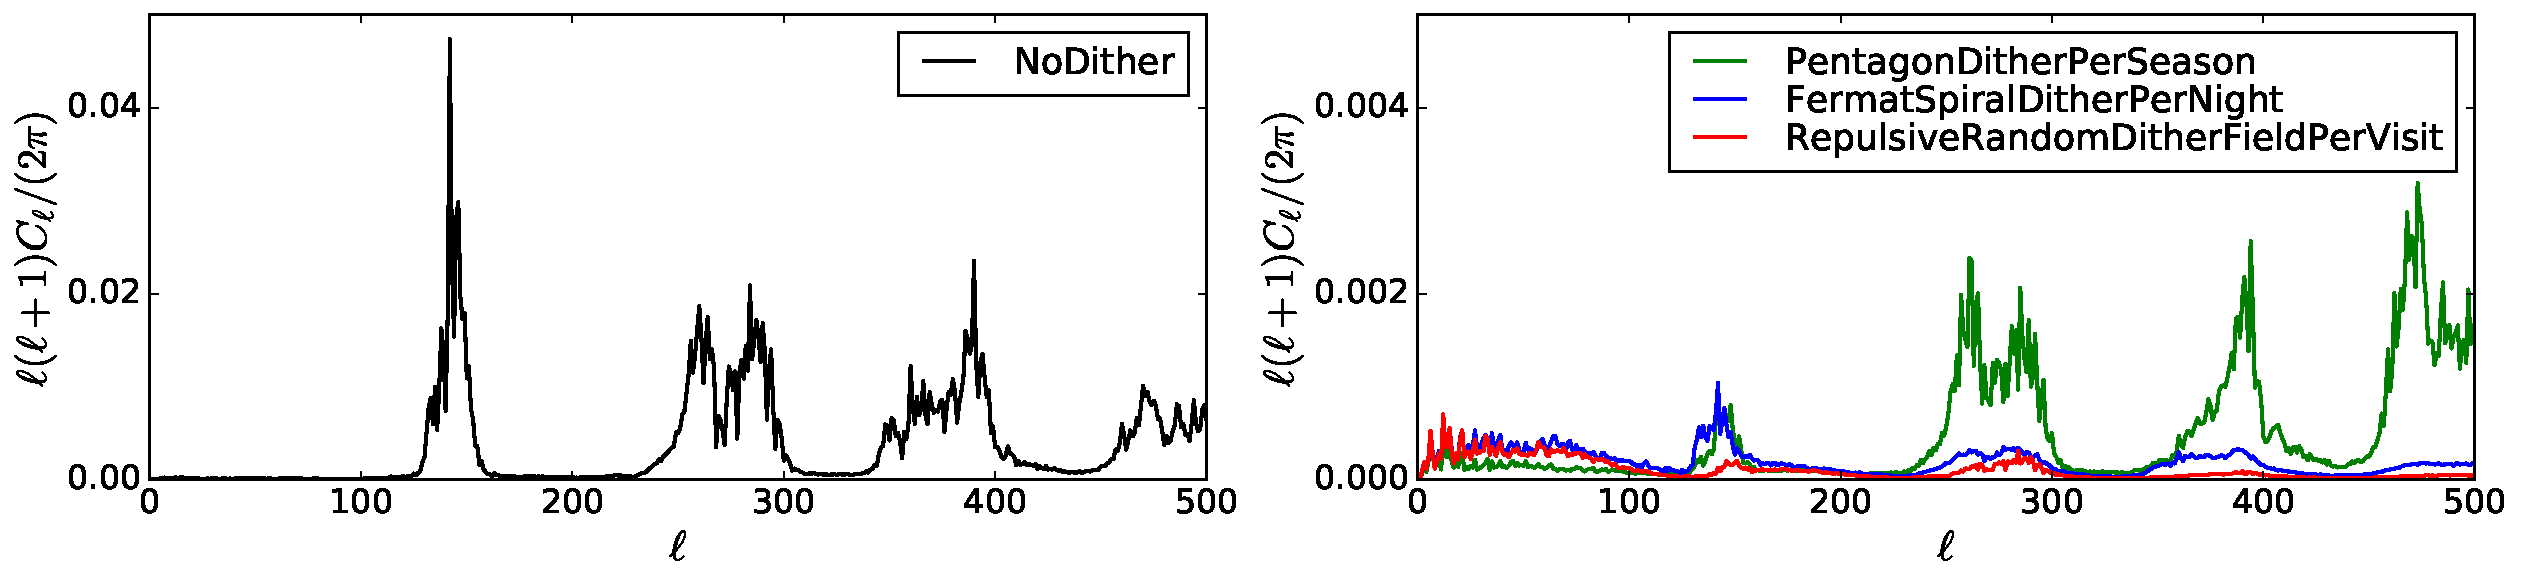
\includegraphics[width=\linewidth]{figs/awan_coaddpowerspectrum.pdf}
      \vspace*{-2em}
\caption{Angular power spectra for the  $i$-band coadded 5$\sigma$ depth from \opsimdbref{db:baseCadence} for various observing strategies. We note that dithering reduces the spurious power by over 10$\times$.}
\label{fig: coaddPowerSpectrum}
\end{figure*}

We then proceed to calculate the OS-induced bias and its uncertainty from the different observing strategies. First, we examine simulated results after only one year of survey. \autoref{fig: minion1016: 1yr} shows the comparison between \sigmaOS\ and \statFloor\ for $0.66<z<1.0$ after the 1-year survey for two magnitude cuts: $i<24.0$ and $i<25.3$. We observe that the undithered survey leads to \sigmaOS\ 1-5$\times$ the statistical floor around $\ell\sim150$; PerSeason timescale does only slightly better. However, we see an improvement with frequent dithers: both FieldPerVisit and PerNight implementations lead to uncertainties 0.5-1$\times$ the statistical floor, although FermatSpiral dithers on PerNight timescale lead to a peak around $\ell\sim150$ more pronounced than the one from RepulsiveRandom dithers on FieldPerVisit timescale.

\begin{figure*}[!htb]
      \centering\hspace*{1em}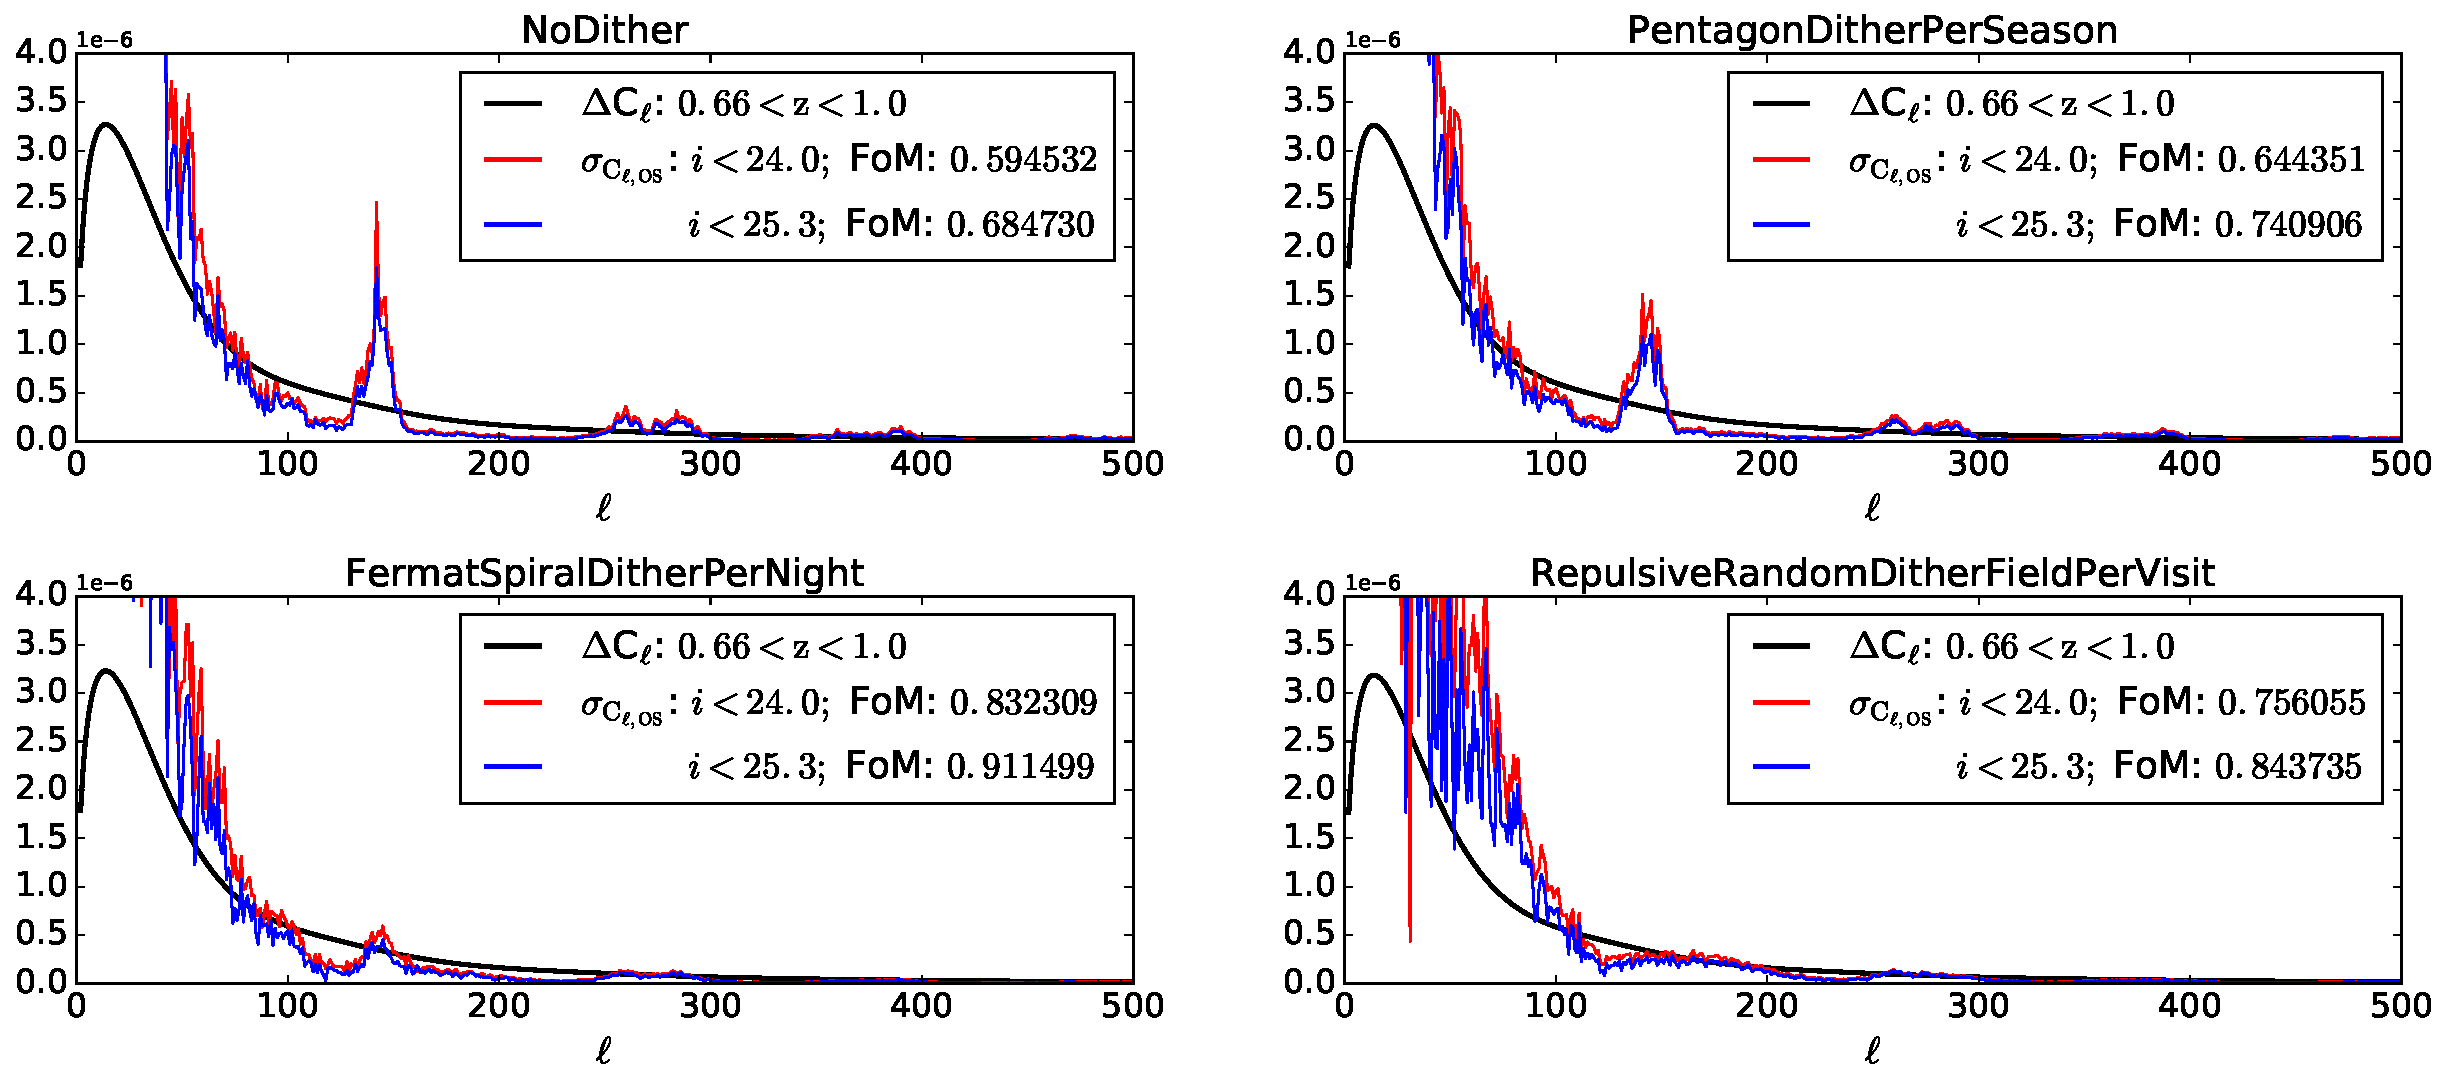
\includegraphics[width=\linewidth]{figs/awan_1yr_minion1016_2magCuts.pdf}
       \vspace*{-2em}
\caption{\sigmaOS\ comparison with the minimum statistical uncertainty \statFloor\ for $0.66<z<1.0$ for different magnitude cuts after only one year of survey based on \opsimdbref{db:baseCadence}.}
\label{fig: minion1016: 1yr}
\end{figure*}

The trends are captured in the Figure of Merit, which we calculate using \autoref{eq: FoM} over the range $100<\ell<300$. We observe a smaller FoM for the shallower survey -- realistic given that although there is less structure and therefore weaker OS-induced artifacts, the shot noise becomes significant and makes the FoM smaller. For the deeper survey, we find that FermatSpiralDitherPerNight outperforms all others with the highest FoM, while RepulsiveRandomDitherFieldPerVisit is more effective than PerSeason dithers. The undithered survey, as expected, performs the worst.

In \autoref{fig: minion1016: 10yr}, we show simulated results after the full, 10-year survey for $0.66<z<1.0$ for three different magnitude cuts: $i<24.0$, $i<25.3$ and $i<27.5$. We observe stark differences between the undithered and dithered surveys: the former leads to large uncertainties in the OS-induced bias while the latter is effective in bringing \sigmaOS\ well below the statistical floor. The effectiveness of all three dithered surveys in minimizing the uncertainties implies more flexibility in choosing the dither strategy for years 2-10.

%For 10yr, 3 magnitude cuts with minion1016, NoDither was always bad but PerSeason dithers were giving us comparable FoM to PerNight and FieldPerVisit dithers. That is not the case anymore; PerSeason dithers are now doing slightly better than before though still not as good as PerNight and FieldPerVisit dithers.

Analyzing the FoM more closely, we observe that the gold sample leads to smaller FoM than both the shallower and deeper catalogs. The larger FoM for shallower catalog is realistic, given less structure with shallow depth leads to weaker artifacts and the shot noise is negligible over the full ten-year survey, but the out-of-trend behavior of gold sample hints at a peculiarity of the variance across the $ugri$ bands at that depth for the baseline cadence. We investigate this behavior briefly and find that the $u$-band-induced artifacts add the most to the uncertainties in the bias induced by the observing strategy, as the gold sample $u$-band cadence in the \opsimdbref{db:baseCadence} is different from $gri$ cadences. This issue still needs to be further investigated, with potentially incorporating the importance of each band to calculate an overall OS-induced bias. We note, however, that this peculiarity is particularly enhanced for the undithered survey.

\begin{figure*}[!htb]
      \centering\hspace*{1em}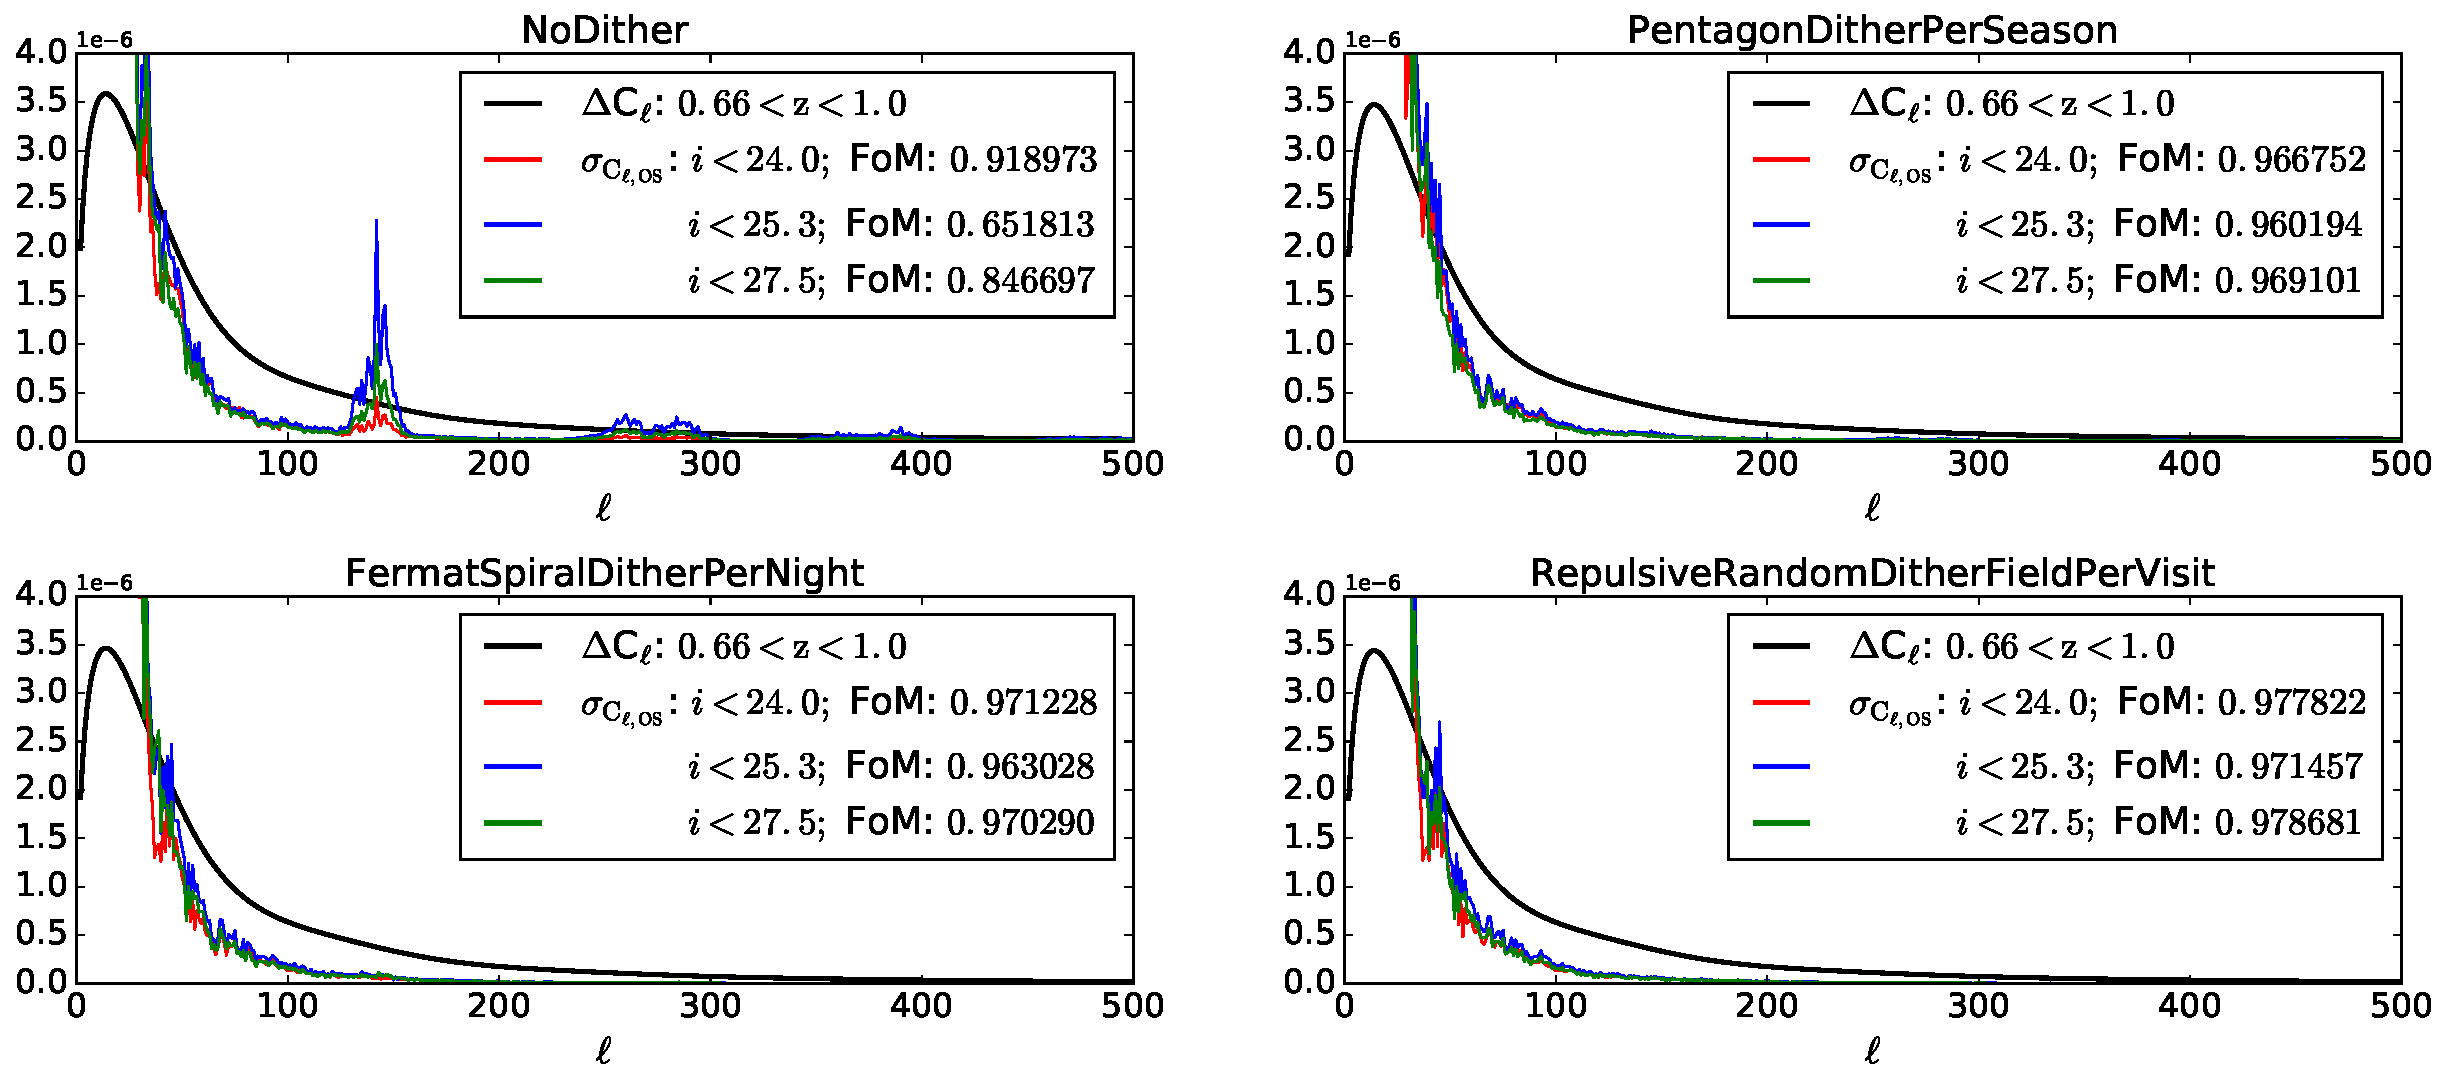
\includegraphics[width=\linewidth]{figs/awan_10yr_minion1016_3magCuts.pdf}
       \vspace*{-2em}
\caption{\sigmaOS\ comparison with the minimum statistical uncertainty \statFloor\ for $0.66<z<1.0$ for different magnitude cuts after the full, 10-year survey based on \opsimdbref{db:baseCadence}.}
\label{fig: minion1016: 10yr}
\end{figure*}

The trends observed here remain consistent for all five redshift bins. We note that our choice of dithers is particularly important for the one-year survey as only one of the three dither strategies leads to a large FoM. Therefore, in the absence of effective dithers, systematics correction methods will become necessary after the one-year survey. However, these methods may not lead to significant improvements for a dithered 10-year survey as dithers of most kinds are effective in reducing the uncertainties well below the minimum statistical limit.

To further probe the effects of dithers, we run the 1-year and 10-year analyses for two cadences besides the baseline cadence: \opsimdbref{db:NoVisitPairs} which does not require visit pairs, and \opsimdbref{db:opstwoPS} which implements a Pan-STARRS-like observing strategy offering a larger area coverage. In \autoref{fig: cadences: 1yr}, we compare the results from these two cadences with those from \opsimdbref{db:baseCadence} for $0.66<z<1.0$ for the  $i<25.3$ galaxy sample after only one year of survey. We see that the undithered survey leads to large uncertainties in the OS-induced bias with all three cadences, with the peak uncertainty 5-15$\times$ the statistical floor. As expected, the undithered survey with the wider coverage \opsimdbref{db:opstwoPS} cadence leads to stronger artifacts and a much smaller FoM (by $\sim33\%$ in comparison with \opsimdbref{db:baseCadence}), while not requiring visit-pairs is slightly more effective than the baseline (FoM increases by about 6$\%$). We see very similar trends for the three cadences for PerSeason dithers although the peak \sigmaOS\ ranges between 3-9$\times$ the statistical floor; FoM based on \opsimdbref{db:opstwoPS} is worse than that from \opsimdbref{db:baseCadence} by about 25$\%$ and  \opsimdbref{db:NoVisitPairs} improves on the baseline FoM by $\sim5\%$.

% For different cadences, 1yr results, we now have FoM really high for the wider minion1020 for both PerNight and FieldPerVisit dithers while NoDither and PerSeason dithers are still performing poorly. RepRandom dithers with the wider survey gets us F0M=0.99 while FermatSpiral dithers perform better than RepRandom for the other two cadences.

As before, \sigmaOS\ improves with more frequent dithering. It is only about 1-3$\times$ the statistical floor for FermatSpiral dithers on PerNight timescale. In contrast to NoDither and PerSeason dithers, both \opsimdbref{db:opstwoPS} and \opsimdbref{db:NoVisitPairs} perform better than baseline\opsimdbref{db:baseCadence} with PerNight dithers: FoM from the wider coverage cadence is about $4.5\%$ better than for the baseline cadence, while we see a $4\%$ better FoM with \opsimdbref{db:NoVisitPairs}. 

For RepulsiveRandom dithers on FieldPerVisit timescale, we find that the uncertainties in the OS-induced bias are on the same scale as the statistical floor. The wider coverage cadence outperforms the baseline cadence significantly as  the wider survey FoM is about $18\%$ better than the baseline FoM while the improvement is about 3$\%$ when not requiring visit-pairs. We emphasize that the differences between results with different cadences is highly dependent on the observing strategy: the wider coverage with no or infrequent dithers performs quite poorly while it significantly improves the FoM when large, frequent dithers are implemented. On the other hand, not requiring visit-pairs leads to comparatively larger improvement for infrequent dithers than frequent ones (compared to the baseline).

\begin{figure*}[!htb]
      \centering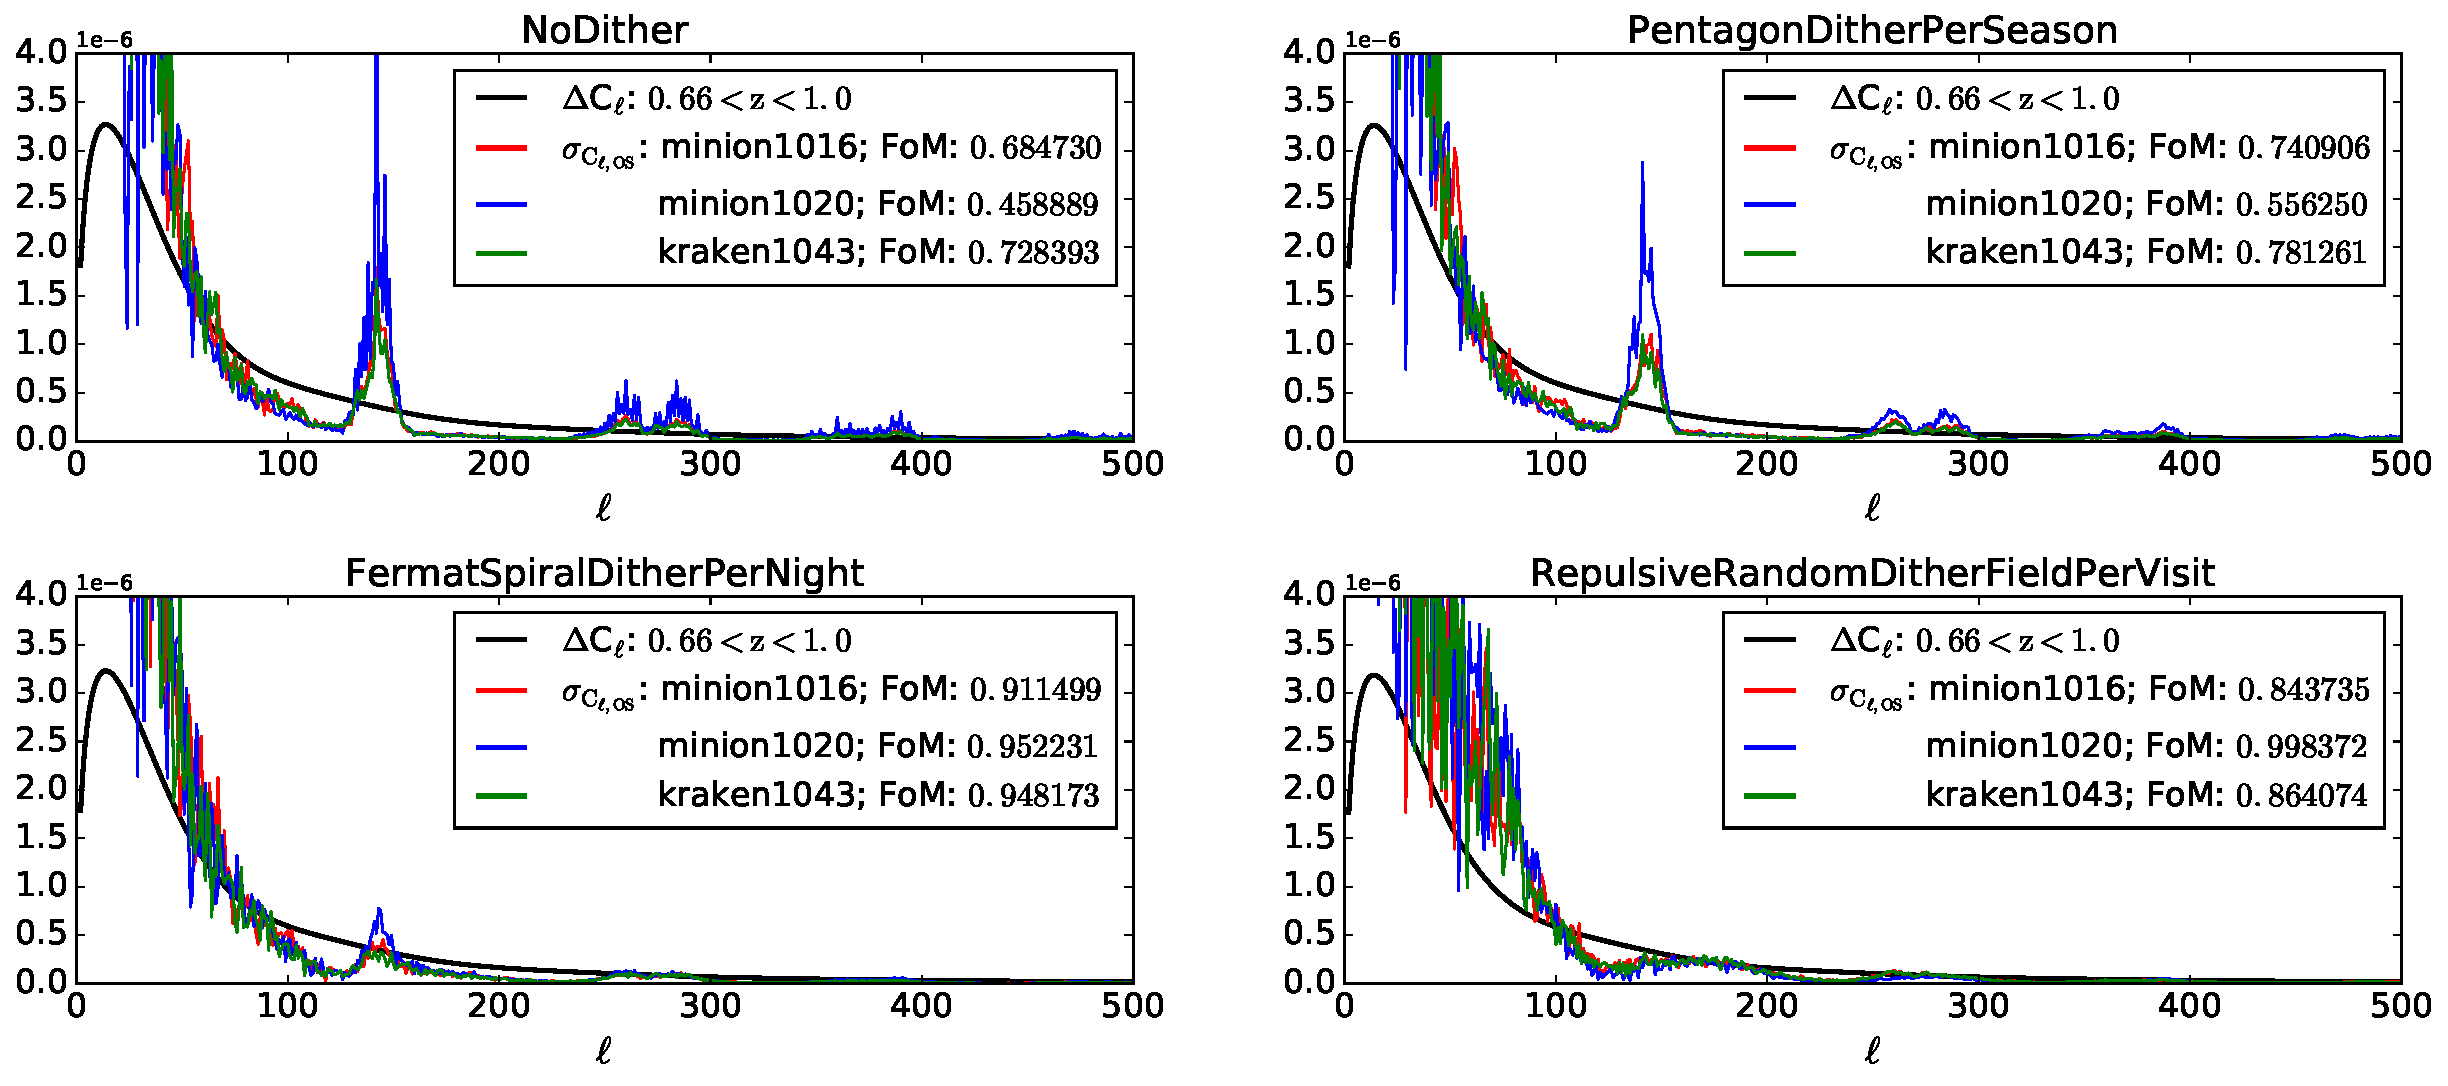
\includegraphics[width=\linewidth]{figs/awan_1yr_goldSample_3cadences.pdf}
       \vspace*{-2em}
\caption{\sigmaOS\ comparison with the minimum statistical uncertainty \statFloor\ for $0.66<z<1.0$ for three different cadences for $i<25.3$ after only one year of survey.}
\label{fig: cadences: 1yr}
\end{figure*}

Finally, we show the simulated results for different cadences after the 10-year survey in \autoref{fig: cadences: 10yr}. As in \autoref{fig: minion1016: 10yr}, we see that all the dithered surveys effectively minimize the uncertainties, regardless of the cadence. We do observe, however, that the wider coverage \opsimdbref{db:opstwoPS} still underperforms significantly for the undithered survey (FoM about 30$\%$ less than baseline FoM)  while all the dithered surveys see a stark improvement (FoM $>$ 1 for all; $\sim 20\%$ improvement on the baseline FoM). The improvement from \opsimdbref{db:NoVisitPairs} is comparable among the four observing strategies. Based on these results, we note than wider coverage offers significant improvements with large dithers on any implementation timescale.

\begin{figure*}[!htb]
      \centering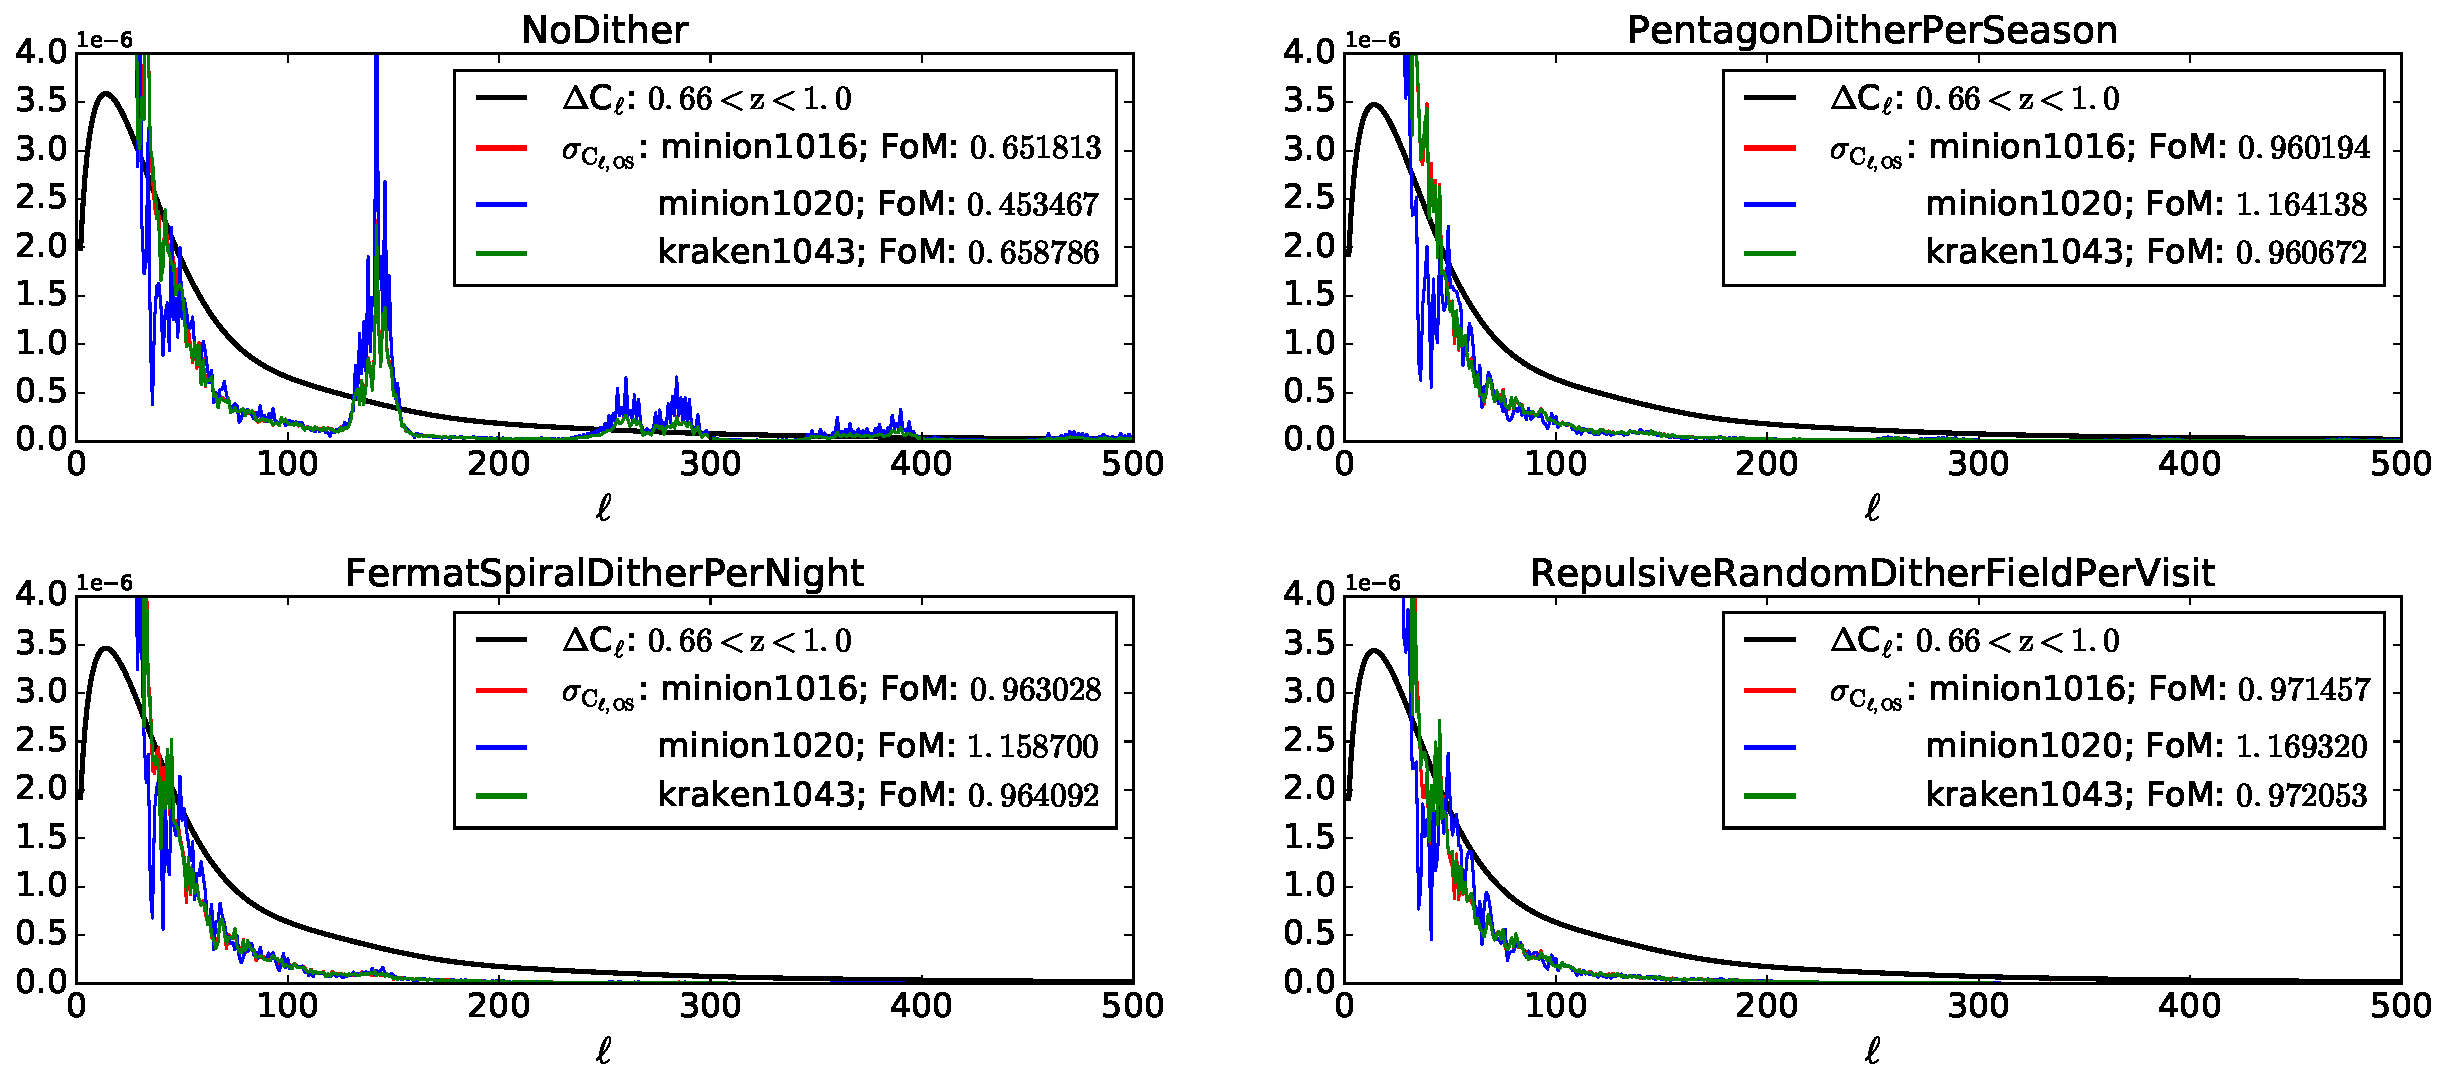
\includegraphics[width=\linewidth]{figs/awan_10yr_goldSample_3cadences.pdf}
       \vspace*{-2em}
\caption{\sigmaOS\ comparison with the minimum statistical uncertainty \statFloor\ for $0.66<z<1.0$ for three different cadences for $i<25.3$ after the full, 10-year survey.}
\label{fig: cadences: 10yr}
\end{figure*}

% ====================================================================
% Science Case Conclusions
% ====================================================================
\subsection{Conclusions}

Here we answer the ten questions posed in
\autoref{sec:intro:evaluation:caseConclusions}:

\begin{description}

\item[Q1:] {\it Does the science case place any constraints on the
tradeoff between the sky coverage and coadded depth? For example, should
the sky coverage be maximized (to $\sim$30,000 deg$^2$, as e.g., in
Pan-STARRS) or the number of detected galaxies (the current baseline but
with 18,000 deg$^2$)?}

\item[A1:] As we see in \autoref{sec:\secname: analysis}, a deeper
catalog is more effective, though it makes the choice of the dither
strategy more important, especially in the first year of survey. We also see 
that the wider-coverage cadence \opsimdbref{db:opstwoPS} performs 
significantly better for LSS systematics with large, frequent dithers  
while it performs much poorly with no or infrequent dithers; this
trend is consistent for both one-year and the full, ten-year surveys. We
note here that one year of the wider coverage (for gold sample) with frequent large
dithers leads to better systematics (as quantized here) than ten years of 
the standard WFD  footprint, strongly supporting the effectiveness of wider area
coverage in the first year of survey for LSS systematics. We are definitely area-
limited more than depth-limited for LSS studies.

\item[Q2:] {\it Does the science case place any constraints on the
tradeoff between uniformity of sampling and frequency of  sampling? For
example, a rolling cadence can provide enhanced sample rates over a part
of the survey or the entire survey for a designated time at the cost of
reduced sample rate the rest of the time (while maintaining the nominal
total visit counts).}

\item[A2:] Depth uniformity is critical for LSS systematics. As we
demonstrated in \autoref{sec:\secname: analysis}, LSS studies will benefit
strongly from large dithers and wide area coverage. We do not have constraints
on the cadence.

\item[Q3:] {\it Does the science case place any constraints on the
tradeoff between the single-visit depth and the number of visits
(especially in the $u$-band where longer exposures would minimize the
impact of the readout noise)?}

\item[A3:] From our investigation into the large uncertainties in the
OS-induced bias observed in the gold sample in the baseline cadence, in
comparison with the shallower and deeper catalogs, we find that
$u$-band-induced artifacts add the most to the uncertainties in the
bias. Hence there could be a significant penalty from reducing the
number of $u$-band visit. At minimum, doing so would make the choice of
dither pattern more important. This issue still needs to be further
investigated.

\item[Q4:] {\it Does the science case place any constraints on the
Galactic plane coverage (spatial coverage, temporal sampling, visits per
band)?}

\item[A4:] LSS systematics do not place any constraints on the Galactic
plane coverage.

\item[Q5:] {\it Does the science case place any constraints on the
fraction of observing time allocated to each band?}

\item[A5:] Increasing the number of visits leads to greater survey
uniformity. At present, this is worst (among $ugri$) in the $u$-band, so
increasing the fraction of $u$-band observing time would likely help.

\item[Q6:] {\it Does the science case place any constraints on the
cadence for deep drilling fields?}

\item[A6:] LSS systematics do not constrain the cadence for deep
drilling fields as long as the main survey dithers are not affected.

\item[Q7:] {\it Assuming two visits per night, would the science case
benefit if they are obtained in the same band or not?}

\item[A7:] We do not see significant difference between obtaining two
visits per night in the same band or not, although we do see a mild
benefit in not obtaining the visits in the same band as it allows
greater variation in atmospheric conditions in each band.

\item[Q8:] {\it Will the case science benefit from a special cadence
prescription during commissioning or early in the survey, such as:
acquiring a full 10-year count of visits for a small area (either in all
the bands or in a  selected set); a greatly enhanced cadence for a small
area?}

\item[A8:] We will request full, 10-year depth during commissioning to
validate our choice of dither pattern.

\item[Q9:] {\it Does the science case place any constraints on the
sampling of observing conditions (e.g., seeing, dark sky, airmass),
possibly as a function of band, etc.?}

\item[A9:] Seeing will play a role in the photometric calibration
errors. However, these errors appear to be subdominant to the artifacts
induced by the observing strategy.

\item[Q10:] {\it Does the case have science drivers that would require
real-time exposure time optimization to obtain nearly constant
single-visit limiting depth?}

\item[A10:] We do not require any real-time exposure time optimization.

\end{description}

% ====================================================================
% Discussion
% ====================================================================
\subsection{Discussion}
\label{sec:\secname:discussion}

In this section, we presented results for the impacts of LSST observing
strategy on LSS studies. Using the OpSim cadence baseline
\opsimdbref{db:baseCadence}, we demonstrate that dithers are necessary
for both 1-year and 10-year surveys. We find that of the three dither strategies
discussed here, FermatSpiral dithers on PerNight  timescale are the most
effective for the gold sample after one-year of survey while  dithers of all kinds
are effective after the ten-year survey. These results imply the need for a very careful
choice of the observing strategy in the first year while there is quite a range of choice 
for years 2-10.

We also analyze two other cadences and find  that frequent dithering with
maximum  sky coverage could allow a significant  fraction LSST-enabled LSS
science after  one-year. Assuming that the quality of photometric redshifts is
fixed (when it actually improves with depth) and that our ansatz for window
function uncertainties is representative,  our results can go as far as implying
that the wider coverage for a few years is far more important than more years of the
baseline  WFD coverage.

Future work will entail improving our analysis to better constrain the
artifacts induced by the observing strategy by, e.g., including
uncertainties in the dust extinction, using improved models for the
photometric calibration uncertainties, more realistic galaxy colors,
incorporating improved mock catalogs to better estimate the galaxy
counts as well as its uncertainties, and a better estimate of the
uncertainties in the OS-induced by a more thorough accounting of the
effects of each band. Also, the development and the analysis of the
effectiveness of various systematics correction methods needs to be
carried out, especially for the 1-year survey, as only a few observing 
strategies reduce the artifacts. Finally, the effectiveness
of various dithers still needs to be assessed for other science probes.


\navigationbar
